\documentclass{standalone}
\usepackage{tikz}
\usetikzlibrary{patterns, positioning}

\begin{document}
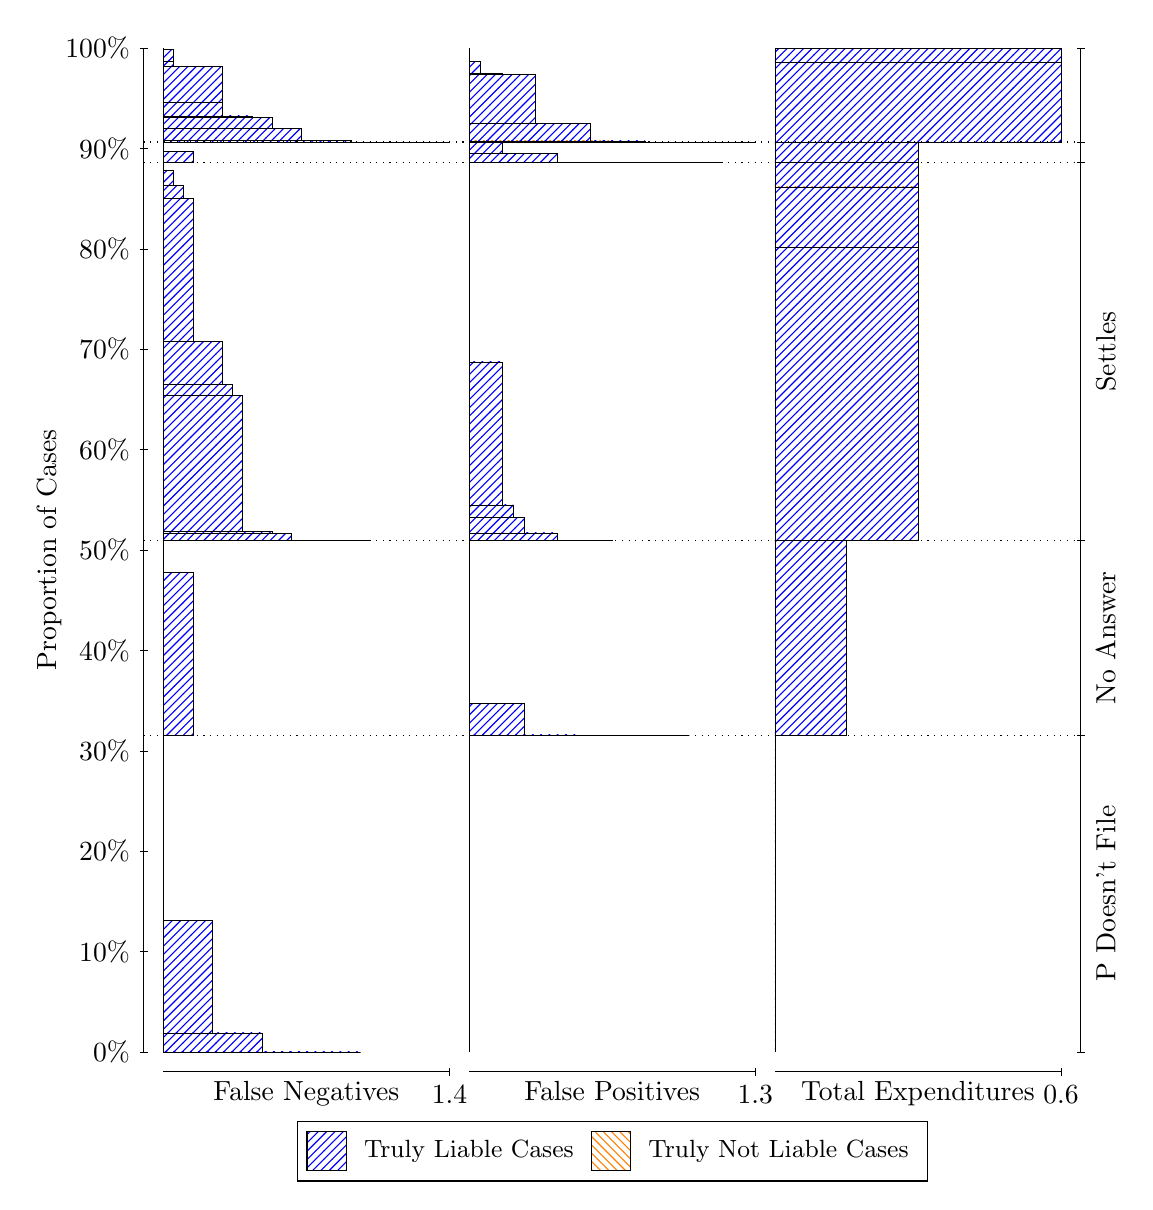
\begin{tikzpicture}
\draw[black, very thin] (1.5,1.75) -- (1.5,14.5);
\node[rotate=90, anchor=center] at (0.3, 8.125) {Proportion of Cases};
\draw[black, very thin] (1.45,1.75) -- (1.55,1.75);
\node[anchor=east] at (1.45, 1.75) {0\%};
\draw[black, very thin] (1.45,3.025) -- (1.55,3.025);
\node[anchor=east] at (1.45, 3.025) {10\%};
\draw[black, very thin] (1.45,4.3) -- (1.55,4.3);
\node[anchor=east] at (1.45, 4.3) {20\%};
\draw[black, very thin] (1.45,5.575) -- (1.55,5.575);
\node[anchor=east] at (1.45, 5.575) {30\%};
\draw[black, very thin] (1.45,6.85) -- (1.55,6.85);
\node[anchor=east] at (1.45, 6.85) {40\%};
\draw[black, very thin] (1.45,8.125) -- (1.55,8.125);
\node[anchor=east] at (1.45, 8.125) {50\%};
\draw[black, very thin] (1.45,9.4) -- (1.55,9.4);
\node[anchor=east] at (1.45, 9.4) {60\%};
\draw[black, very thin] (1.45,10.675) -- (1.55,10.675);
\node[anchor=east] at (1.45, 10.675) {70\%};
\draw[black, very thin] (1.45,11.95) -- (1.55,11.95);
\node[anchor=east] at (1.45, 11.95) {80\%};
\draw[black, very thin] (1.45,13.225) -- (1.55,13.225);
\node[anchor=east] at (1.45, 13.225) {90\%};
\draw[black, very thin] (1.45,14.5) -- (1.55,14.5);
\node[anchor=east] at (1.45, 14.5) {100\%};

\draw[black, very thin] (13.4,1.75) -- (13.4,14.5);
\draw[black, very thin] (13.35,1.75) -- (13.45,1.75);
\node[anchor=west] at (13.35, 1.75) {};
\draw[black, very thin] (13.35,5.7734) -- (13.45,5.7734);
\node[anchor=west] at (13.35, 5.7734) {};
\draw[black, very thin] (13.35,8.2469) -- (13.45,8.2469);
\node[anchor=west] at (13.35, 8.2469) {};
\draw[black, very thin] (13.35,13.045) -- (13.45,13.045);
\node[anchor=west] at (13.35, 13.045) {};
\draw[black, very thin] (13.35,13.306) -- (13.45,13.306);
\node[anchor=west] at (13.35, 13.306) {};
\draw[black, very thin] (13.35,14.5) -- (13.45,14.5);
\node[anchor=west] at (13.35, 14.5) {};

\draw[black, very thin, pattern color=blue, pattern=north east lines] (1.75,1.75) rectangle (4.2557,1.75);
\draw[black, very thin, pattern color=blue, pattern=north east lines] (1.75,1.75) rectangle (3.6293,1.752);
\draw[black, very thin, pattern color=blue, pattern=north east lines] (1.75,1.752) rectangle (3.0029,1.9923);
\draw[black, very thin, pattern color=blue, pattern=north east lines] (1.75,1.9923) rectangle (2.3764,3.4228);
\draw[black, very thin, pattern color=orange, pattern=north west lines] (1.75,3.4228) rectangle (1.75,3.4228);
\draw[black, very thin, pattern color=blue, pattern=north east lines] (1.75,3.4228) rectangle (1.75,5.7734);
\draw[black, very thin, pattern color=blue, pattern=north east lines] (1.75,5.7734) rectangle (2.1259,7.8425);
\draw[black, very thin, pattern color=orange, pattern=north west lines] (1.75,7.8425) rectangle (1.75,7.8425);
\draw[black, very thin, pattern color=blue, pattern=north east lines] (1.75,7.8425) rectangle (1.75,8.2469);
\draw[black, very thin, pattern color=blue, pattern=north east lines] (1.75,8.2469) rectangle (4.381,8.2469);
\draw[black, very thin, pattern color=blue, pattern=north east lines] (1.75,8.2469) rectangle (3.8799,8.2469);
\draw[black, very thin, pattern color=blue, pattern=north east lines] (1.75,8.2469) rectangle (3.7546,8.2469);
\draw[black, very thin, pattern color=blue, pattern=north east lines] (1.75,8.2469) rectangle (3.3787,8.333);
\draw[black, very thin, pattern color=blue, pattern=north east lines] (1.75,8.333) rectangle (3.2534,8.3342);
\draw[black, very thin, pattern color=blue, pattern=north east lines] (1.75,8.3342) rectangle (3.1282,8.3576);
\draw[black, very thin, pattern color=blue, pattern=north east lines] (1.75,8.3576) rectangle (2.7523,10.086);
\draw[black, very thin, pattern color=blue, pattern=north east lines] (1.75,10.086) rectangle (2.627,10.227);
\draw[black, very thin, pattern color=blue, pattern=north east lines] (1.75,10.227) rectangle (2.5017,10.778);
\draw[black, very thin, pattern color=blue, pattern=north east lines] (1.75,10.778) rectangle (2.1259,12.594);
\draw[black, very thin, pattern color=blue, pattern=north east lines] (1.75,12.594) rectangle (2.0006,12.757);
\draw[black, very thin, pattern color=blue, pattern=north east lines] (1.75,12.757) rectangle (1.8753,12.949);
\draw[black, very thin, pattern color=orange, pattern=north west lines] (1.75,12.949) rectangle (1.75,12.949);
\draw[black, very thin, pattern color=blue, pattern=north east lines] (1.75,12.949) rectangle (1.75,13.045);
\draw[black, very thin, pattern color=blue, pattern=north east lines] (1.75,13.045) rectangle (2.1259,13.185);
\draw[black, very thin, pattern color=orange, pattern=north west lines] (1.75,13.185) rectangle (1.75,13.185);
\draw[black, very thin, pattern color=blue, pattern=north east lines] (1.75,13.185) rectangle (1.75,13.306);
\draw[black, very thin, pattern color=blue, pattern=north east lines] (1.75,13.306) rectangle (5.3833,13.306);
\draw[black, very thin, pattern color=blue, pattern=north east lines] (1.75,13.306) rectangle (4.7569,13.306);
\draw[black, very thin, pattern color=blue, pattern=north east lines] (1.75,13.306) rectangle (4.381,13.306);
\draw[black, very thin, pattern color=blue, pattern=north east lines] (1.75,13.306) rectangle (4.1305,13.328);
\draw[black, very thin, pattern color=blue, pattern=north east lines] (1.75,13.328) rectangle (3.7546,13.328);
\draw[black, very thin, pattern color=blue, pattern=north east lines] (1.75,13.328) rectangle (3.504,13.475);
\draw[black, very thin, pattern color=blue, pattern=north east lines] (1.75,13.475) rectangle (3.1282,13.624);
\draw[black, very thin, pattern color=blue, pattern=north east lines] (1.75,13.624) rectangle (2.8776,13.637);
\draw[black, very thin, pattern color=blue, pattern=north east lines] (1.75,13.637) rectangle (2.5017,13.806);
\draw[black, very thin, pattern color=blue, pattern=north east lines] (1.75,13.806) rectangle (2.5017,14.266);
\draw[black, very thin, pattern color=blue, pattern=north east lines] (1.75,14.266) rectangle (2.2511,14.266);
\draw[black, very thin, pattern color=blue, pattern=north east lines] (1.75,14.266) rectangle (1.8753,14.336);
\draw[black, very thin, pattern color=blue, pattern=north east lines] (1.75,14.336) rectangle (1.8753,14.485);
\draw[black, very thin, pattern color=orange, pattern=north west lines] (1.75,14.485) rectangle (1.75,14.485);
\draw[black, very thin, pattern color=blue, pattern=north east lines] (1.75,14.485) rectangle (1.75,14.5);
\draw[black, very thin, pattern color=orange, pattern=north west lines] (5.6333,1.75) rectangle (5.6333,1.75);
\draw[black, very thin, pattern color=blue, pattern=north east lines] (5.6333,1.75) rectangle (5.6333,5.7734);
\draw[black, very thin, pattern color=orange, pattern=north west lines] (5.6333,5.7734) rectangle (8.4282,5.7734);
\draw[black, very thin, pattern color=blue, pattern=north east lines] (5.6333,5.7734) rectangle (8.4282,5.7734);
\draw[black, very thin, pattern color=blue, pattern=north east lines] (5.6333,5.7734) rectangle (7.7295,5.7734);
\draw[black, very thin, pattern color=blue, pattern=north east lines] (5.6333,5.7734) rectangle (7.0308,5.7765);
\draw[black, very thin, pattern color=blue, pattern=north east lines] (5.6333,5.7765) rectangle (6.3321,6.1779);
\draw[black, very thin, pattern color=blue, pattern=north east lines] (5.6333,6.1779) rectangle (5.6333,8.2469);
\draw[black, very thin, pattern color=orange, pattern=north west lines] (5.6333,8.2469) rectangle (7.45,8.2469);
\draw[black, very thin, pattern color=blue, pattern=north east lines] (5.6333,8.2469) rectangle (7.45,8.247);
\draw[black, very thin, pattern color=orange, pattern=north west lines] (5.6333,8.247) rectangle (6.891,8.247);
\draw[black, very thin, pattern color=blue, pattern=north east lines] (5.6333,8.247) rectangle (6.891,8.2511);
\draw[black, very thin, pattern color=blue, pattern=north east lines] (5.6333,8.2511) rectangle (6.7513,8.3437);
\draw[black, very thin, pattern color=orange, pattern=north west lines] (5.6333,8.3437) rectangle (6.3321,8.3437);
\draw[black, very thin, pattern color=blue, pattern=north east lines] (5.6333,8.3437) rectangle (6.3321,8.535);
\draw[black, very thin, pattern color=blue, pattern=north east lines] (5.6333,8.535) rectangle (6.1923,8.6984);
\draw[black, very thin, pattern color=blue, pattern=north east lines] (5.6333,8.6984) rectangle (6.0526,10.514);
\draw[black, very thin, pattern color=blue, pattern=north east lines] (5.6333,10.514) rectangle (5.6333,13.045);
\draw[black, very thin, pattern color=orange, pattern=north west lines] (5.6333,13.045) rectangle (8.8474,13.045);
\draw[black, very thin, pattern color=blue, pattern=north east lines] (5.6333,13.045) rectangle (8.8474,13.045);
\draw[black, very thin, pattern color=blue, pattern=north east lines] (5.6333,13.045) rectangle (8.1487,13.045);
\draw[black, very thin, pattern color=blue, pattern=north east lines] (5.6333,13.045) rectangle (7.45,13.047);
\draw[black, very thin, pattern color=blue, pattern=north east lines] (5.6333,13.047) rectangle (6.7513,13.166);
\draw[black, very thin, pattern color=blue, pattern=north east lines] (5.6333,13.166) rectangle (6.0526,13.306);
\draw[black, very thin, pattern color=orange, pattern=north west lines] (5.6333,13.306) rectangle (9.2667,13.306);
\draw[black, very thin, pattern color=blue, pattern=north east lines] (5.6333,13.306) rectangle (9.2667,13.306);
\draw[black, very thin, pattern color=orange, pattern=north west lines] (5.6333,13.306) rectangle (8.5679,13.306);
\draw[black, very thin, pattern color=blue, pattern=north east lines] (5.6333,13.306) rectangle (8.5679,13.306);
\draw[black, very thin, pattern color=orange, pattern=north west lines] (5.6333,13.306) rectangle (7.8692,13.306);
\draw[black, very thin, pattern color=blue, pattern=north east lines] (5.6333,13.306) rectangle (7.8692,13.32);
\draw[black, very thin, pattern color=orange, pattern=north west lines] (5.6333,13.32) rectangle (7.45,13.32);
\draw[black, very thin, pattern color=blue, pattern=north east lines] (5.6333,13.32) rectangle (7.45,13.32);
\draw[black, very thin, pattern color=orange, pattern=north west lines] (5.6333,13.32) rectangle (7.1705,13.32);
\draw[black, very thin, pattern color=blue, pattern=north east lines] (5.6333,13.32) rectangle (7.1705,13.54);
\draw[black, very thin, pattern color=orange, pattern=north west lines] (5.6333,13.54) rectangle (6.7513,13.54);
\draw[black, very thin, pattern color=blue, pattern=north east lines] (5.6333,13.54) rectangle (6.7513,13.54);
\draw[black, very thin, pattern color=blue, pattern=north east lines] (5.6333,13.54) rectangle (6.4718,14.169);
\draw[black, very thin, pattern color=blue, pattern=north east lines] (5.6333,14.169) rectangle (6.0526,14.179);
\draw[black, very thin, pattern color=orange, pattern=north west lines] (5.6333,14.179) rectangle (6.0526,14.179);
\draw[black, very thin, pattern color=blue, pattern=north east lines] (5.6333,14.179) rectangle (6.0526,14.181);
\draw[black, very thin, pattern color=blue, pattern=north east lines] (5.6333,14.181) rectangle (5.7731,14.331);
\draw[black, very thin, pattern color=blue, pattern=north east lines] (5.6333,14.331) rectangle (5.6333,14.5);
\draw[black, very thin, pattern color=orange, pattern=north west lines] (9.5167,1.75) rectangle (9.5167,1.75);
\draw[black, very thin, pattern color=blue, pattern=north east lines] (9.5167,1.75) rectangle (9.5167,5.7734);
\draw[black, very thin, pattern color=orange, pattern=north west lines] (9.5167,5.7734) rectangle (10.425,5.7734);
\draw[black, very thin, pattern color=blue, pattern=north east lines] (9.5167,5.7734) rectangle (10.425,8.2469);
\draw[black, very thin, pattern color=orange, pattern=north west lines] (9.5167,8.2469) rectangle (11.333,8.2469);
\draw[black, very thin, pattern color=blue, pattern=north east lines] (9.5167,8.2469) rectangle (11.333,11.97);
\draw[black, very thin, pattern color=orange, pattern=north west lines] (9.5167,11.97) rectangle (11.333,11.97);
\draw[black, very thin, pattern color=blue, pattern=north east lines] (9.5167,11.97) rectangle (11.333,12.736);
\draw[black, very thin, pattern color=orange, pattern=north west lines] (9.5167,12.736) rectangle (11.333,12.736);
\draw[black, very thin, pattern color=blue, pattern=north east lines] (9.5167,12.736) rectangle (11.333,13.045);
\draw[black, very thin, pattern color=orange, pattern=north west lines] (9.5167,13.045) rectangle (11.333,13.045);
\draw[black, very thin, pattern color=blue, pattern=north east lines] (9.5167,13.045) rectangle (11.333,13.306);
\draw[black, very thin, pattern color=orange, pattern=north west lines] (9.5167,13.306) rectangle (13.15,13.306);
\draw[black, very thin, pattern color=blue, pattern=north east lines] (9.5167,13.306) rectangle (13.15,14.319);
\draw[black, very thin, pattern color=orange, pattern=north west lines] (9.5167,14.319) rectangle (13.15,14.319);
\draw[black, very thin, pattern color=blue, pattern=north east lines] (9.5167,14.319) rectangle (13.15,14.5);
\draw[black, dotted] (1.5,5.7734) -- (13.4,5.7734);
\draw[black, dotted] (1.5,8.2469) -- (13.4,8.2469);
\draw[black, dotted] (1.5,13.045) -- (13.4,13.045);
\draw[black, dotted] (1.5,13.306) -- (13.4,13.306);
\draw[black, very thin] (1.75,1.5) -- (5.3833,1.5);
\node[anchor=north] at (3.5667, 1.5) {False Negatives};
\draw[black, very thin] (5.3833,1.45) -- (5.3833,1.55);
\node[anchor=north] at (5.3833, 1.45) {1.4};

\draw[black, very thin] (5.6333,1.5) -- (9.2667,1.5);
\node[anchor=north] at (7.45, 1.5) {False Positives};
\draw[black, very thin] (9.2667,1.45) -- (9.2667,1.55);
\node[anchor=north] at (9.2667, 1.45) {1.3};

\draw[black, very thin] (9.5167,1.5) -- (13.15,1.5);
\node[anchor=north] at (11.333, 1.5) {Total Expenditures};
\draw[black, very thin] (13.15,1.45) -- (13.15,1.55);
\node[anchor=north] at (13.15, 1.45) {0.6};

\node[black, centered, rotate=90] at (13.72, 3.7617) {P Doesn't File};
\node[black, centered, rotate=90] at (13.72, 7.0102) {No Answer};
\node[black, centered, rotate=90] at (13.72, 10.646) {Settles};



\draw (7.449999999999999,1.5) node[draw=none] (baseCoordinate) {};
\begin{scope}[align=center]
        \matrix[scale=0.5, draw=black, below=0.5cm of baseCoordinate, nodes={draw}, column sep=0.1cm]{
            \node[rectangle, draw, minimum width=0.5cm, minimum height=0.5cm, pattern=north east lines, pattern color=blue] {}; &
            \node[draw=none, font=\small] (B) {Truly Liable Cases}; &
            \node[rectangle, draw, minimum width=0.5cm, minimum height=0.5cm, pattern=north west lines, pattern color=orange] {}; &
            \node[draw=none, font=\small] (B) {Truly Not Liable Cases}; \\
            };
\end{scope}

\end{tikzpicture}
\end{document}